\section{Memory consistency models (\mcms)}\label{sec:cons}
In order to create a mapping from memory consistency models (\mcms) to the \rts\ we need to establish a formalism for the \mcms. In this section, we use the formalism of Alglave \etal\cite{Alglave:2014} to describe \emph{synchronization patterns} (\synpats) and assert that any \mcm\ $CM$ is defined as a set of \synpats\ $S_{CM}$. An execution enforces $CM$ iff it enforces every \synpat\ in $S_{CM}$.
Below we define what a \synpat\ is and what its enforcement entails. 






\begin{table}[t]
\centering
\resizebox{0.48\textwidth}{!}{
\begin{tabular}{|c|||c|||c|}
\hline
\colorhl\textbf{po-type}  & 
\colorhl\textbf{syn-type}&
\colorhl\textbf{hb -type}  
\\ 
\hline
\hline
$\poww$ $\triangleq$
$po \cap WW$ 
&
$ws$  $\triangleq$ 
$syn \cap WW$
&
$\hbww$ $\triangleq$ 
$hb \cap WW$ 
\\ \hline 

$\powr$ $\triangleq$ 
$po \cap WR$ 
&
$syn_{wr}$ $\triangleq$
$syn \cap WR$
&
$\hbwr$ $\triangleq$ 
$hb \cap WR$\\
\hline 

$\porr$ $\triangleq$ 
$po \cap RR$ 
&
$syn_{rr}$ $\triangleq$
$syn \cap RR$
&
$\hbrr$ $\triangleq$ 
$hb \cap RR$\\ \hline 

$\porw$ $\triangleq$ 
$po \cap RW$ 
&
$fr$ $\triangleq$ 
$syn \cap RW$
&
$\hbrw$ $\triangleq$ 
$hb \cap RW$\\ \hline 


\end{tabular}}
\caption{The types of po, syn and hb relations}
\label{tab:posyn}
\end{table}
\begin{figure}[t]
  \centering
  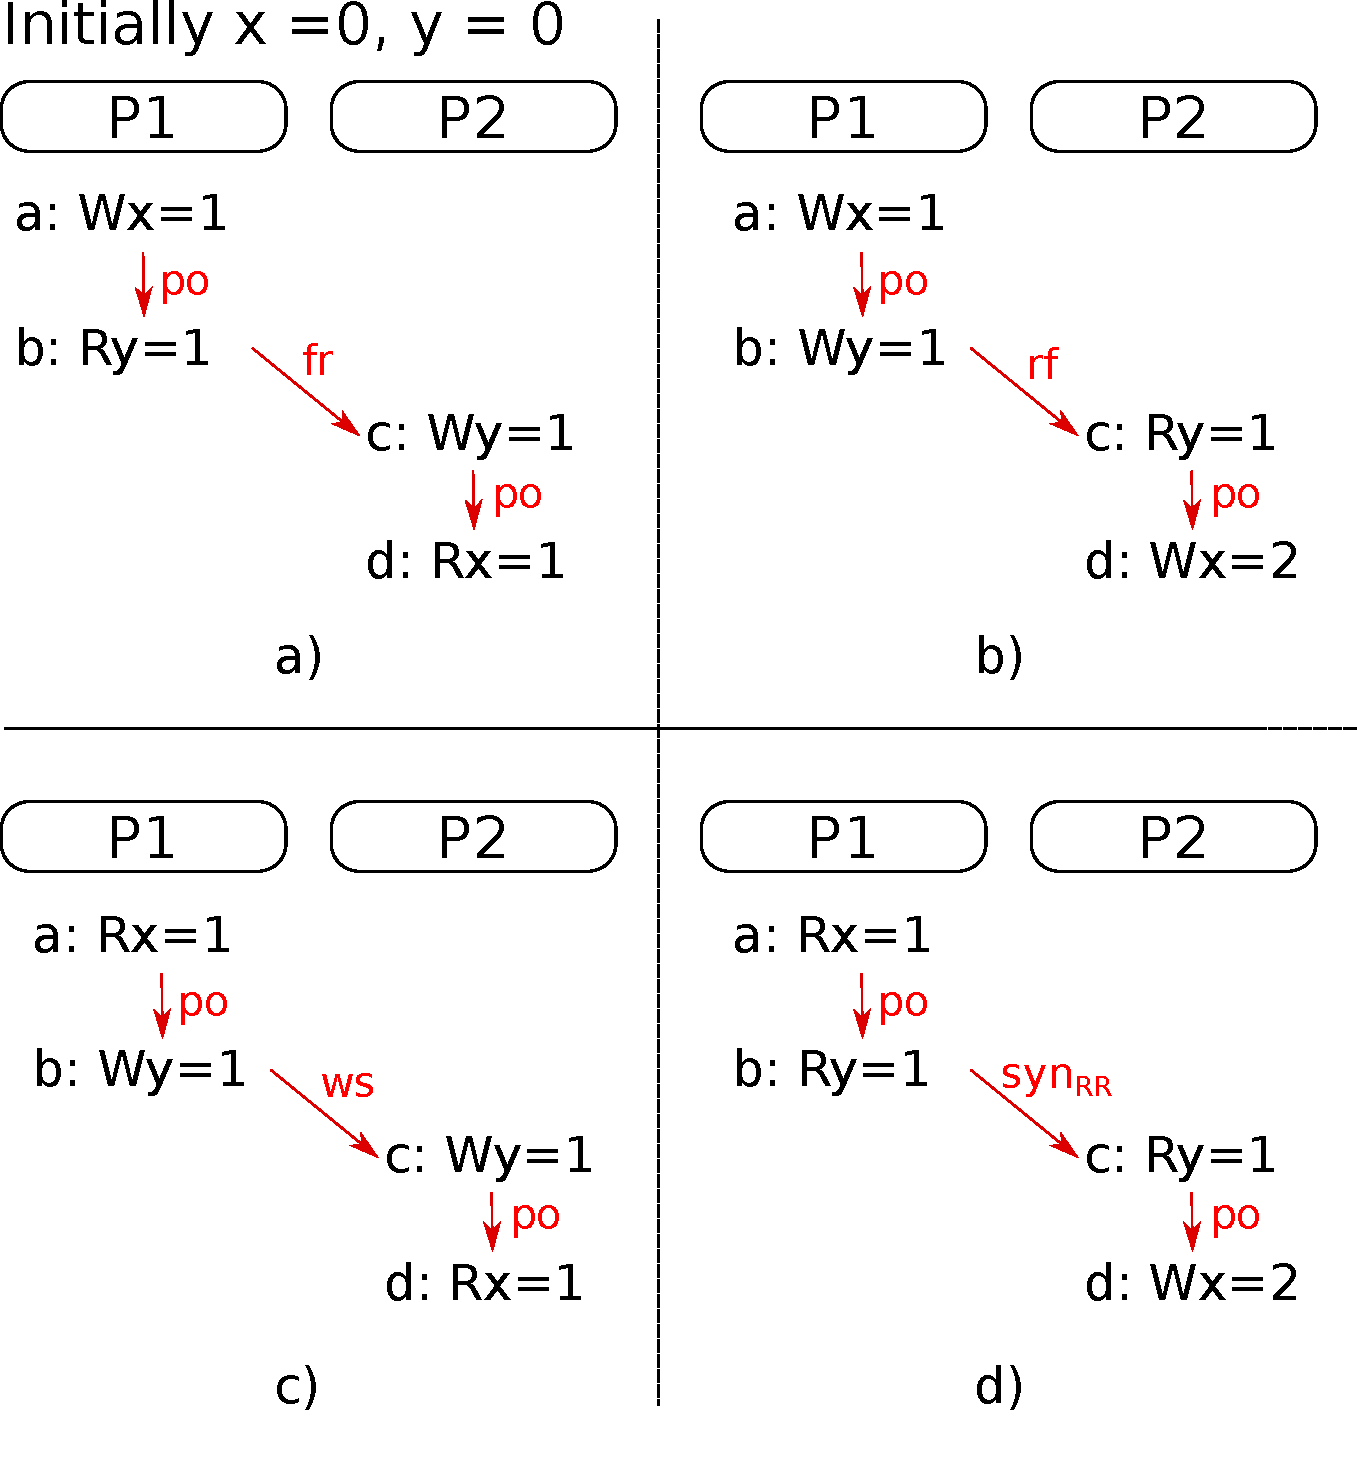
\includegraphics[width=0.28\textwidth]{1_figures/synpat-examples.pdf} 
  \caption{Four examples of \synpats}
  \label{fig:synpat}
\end{figure}


A \synpat\ is a path between two operations to the same object. The path can be constructed through any composition of $\potype$ and $\syntype$ relations, with the only restriction being that at least one $\potype$ must be included (explained in the remarks below).
\tabref{tab:posyn} describes which relations are denoted $\potype$ and $\syntype$.

For example, consider the \synpat\ $s$ that consists of a $\powr$ relation, then an $fr$ relation and then a $\powr$ (depicted in \figref{fig:synpat}a).
We can describe $s$ by composing the three relations as follows:
\begin{equation*}
    s \triangleq \powr ; fr ; \powr
\end{equation*}

Given an execution $E (M, po, rf, hb, RL)$, we assert that $E$ \emph{enforces} $s$ if there exists $rl \in RL$ from which we can derive a $syn$ such that:
\begin{equation*}
    acyclic(s \cup syn)
\end{equation*}
In other words, a \synpat\ that starts from operation $a$ and ends on operation $b$ is said to be \emph{enforced} if $(b, a) \notin syn$.  


\figref{fig:synpat} depicts four \synpats\ to serve as examples.
In the execution of \figref{fig:synpat}a, the $s$ \synpat\ occurs between 
operations $a$ and  $d$. In this instance, $s$ is enforced because $d$ returns the value created by $a$.
If $d$ were to return $0$, that would mean that there is a $syn$ relation between $d$ and $a$ and thus $s$ is not enforced.

\beginbsec{Remarks}
Note the following two remarks. 
First, we use $syn$ rather than $rl$ to test whether a \synpat\ is enforced. This is because the \synpat\ is a path between two operations to the same object, but $rl$ is a total order of all operations across all objects.
Second, note that a \synpat\ must have at least one $\potype$, because otherwise it would just be a composition of $\syntype$ relations. Any such composition is a subset of $syn$, which means that the execution enforces it by definition.

\beginbsec{Consistency models}
An \mcm\ $CM_i$ is defined by asserting that a set
of \synpats\ $S_{CM}$ must be enforced. Plainly, an execution enforces $CM_i$ iff it enforces every $s \in S_{CM}$
As an example, assume that $CM_i$ is defined through the four \synpats\  depicted in \figref{fig:synpat}, which are formalized as follows:
\begin{gather*}
    s_1 \triangleq \powr ; fr ; \powr, \
    s_2 \triangleq \poww ; rf ; \porw, \\
    s_3 \triangleq \porw ; ws ; \powr, \
    s_4 \triangleq \porr ; \synrr ; \porw
\end{gather*}

We define $CM_i$ to be the following rule:
\begin{gather*}
    acyclic(s_1 \cup syn)\
    \andm\ acyclic(s_2 \cup syn)\\ 
    \andm\ acyclic(s_3 \cup syn)\ 
    \andm\ acyclic(s_4 \cup syn)
\end{gather*}




